\section{Dataset generation}
\subsection{Tested approaches}
The deep learning approaches applied in this work are \emph{supervised learning} techniques that require a labeled dataset. Many attempts were made in order to generate a high-quality labeled dataset for the deep learning models:
\begin{itemize}
    \item \emph{IMU sensors}: usage of gyroscope and accelerometer sensors of a smartphone to estimate the position of the camera during a video given a fixed origin point. The process of combining multiple noisy information sources to obtain a good estimation can be achieved through Kalman filters;
    \item \emph{digital video}: usage of free online 3 dimensional datasets in which video can be recorder in a digital way;
    \item \emph{motion capture system}: usage of a motion capture system that estimates the camera position following some tracking objects attached to the subject;
    \item \emph{structure from motion}: techniques that digitally reconstruct environments from a sequence of images with point clouds.
\end{itemize}

The main problem encountered with IMU sensors is the high presence of noise during data acquisition: this causes the processed signal to be very dirty, so much that the precision is not acceptable for our intentions. A possible solution should imply exploiting some well calibrated hardware in a controlled environment.

Most of the online-available 3D acquisitions are acquired with \emph{depth sensors} or \emph{LIDAR sensors}. For this reason, although the camera pose estimation would have been very precise, we could not reproduce this acquisition system in the University of Trento. In addition to that, only few datasets are freely available, and they usually lack of good documentation regarding how they were captured.

The motion capture system is able to follow the position of the tracked objects with extreme precision. In this case the main problems are related to the association of poses to video captured from the camera held by the tracked subject and difficulties involved in the system calibration.

The techniques of structure from motion are used to generate 3D models in case many photos are available. The overall idea is to feed the algorithm with these images in order to extract features and build a recomposition of the environment through a point cloud.
During the reconstruction process, structure from motion tools also compute camera poses in an arbitrary reference system: this intermediate requirement have been exploited by us to generate a labeled dataset, as presented in \cref{fig:trajectory-colmap}.

\begin{figure}[htbp]
    \begin{center}
        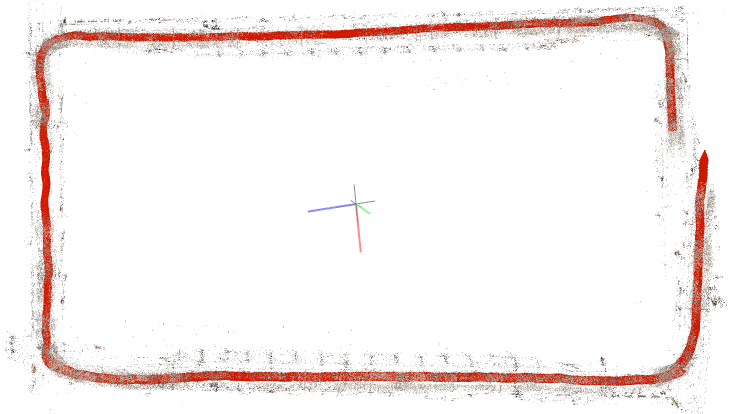
\includegraphics[width=0.45\textwidth]{./imgs/trajectory_colmap.png}
    \end{center}
    \caption{Trajectory computed by a structure from motion algorithm (COLMAP) in the second floor of the Povo 1 building in the University of Trento. Note that these techniques may not detect successfully closed-loops.}
    \label{fig:trajectory-colmap}
\end{figure}

\subsection{Pipeline}
In this section we present an automatic pipeline to generate a labeled camera pose estimation dataset using structure from motion technique. The pipeline requires as input a video captured by any camera, even without sensor calibration. It is composed by several steps:
\begin{enumerate}
    \item video split: the captured video is split into many frames using \texttt{ffmpeg};
    \item structure from motion: frames obtained from the previous step are fed into a structure motion tool that estimates camera poses. In our case we are using \texttt{COLMAP}~\cite{colmap};
    \item dataset splitting: poses computed in the previous step are split into three subsets: train, validation, and test.
\end{enumerate}

\subsection{COLMAP reconstruction}
COLMAP~\cite{colmap} is a tool that allows to build a 3D points clouds reconstruction model of an environment by using photos of it.
Like the other structure from motion techniques, COLMAP also computes camera poses in an arbitrary reference system during the reconstruction process.
It is possible to generate point clouds with two different levels of precision: \emph{sparse} and \emph{dense}, and both of them are composed by:
\begin{itemize}
    \item a set of points $P$ which represent the features extracted from the photos (points in \cref{fig:features-colmap});
    \item a set of poses $\mathcal{V}$ associated with the images used for the reconstruction (red line in \cref{fig:features-colmap});
    \item a \emph{coordinate reference system} (CRS).
\end{itemize}

\begin{figure}[htbp]
    \begin{center}
        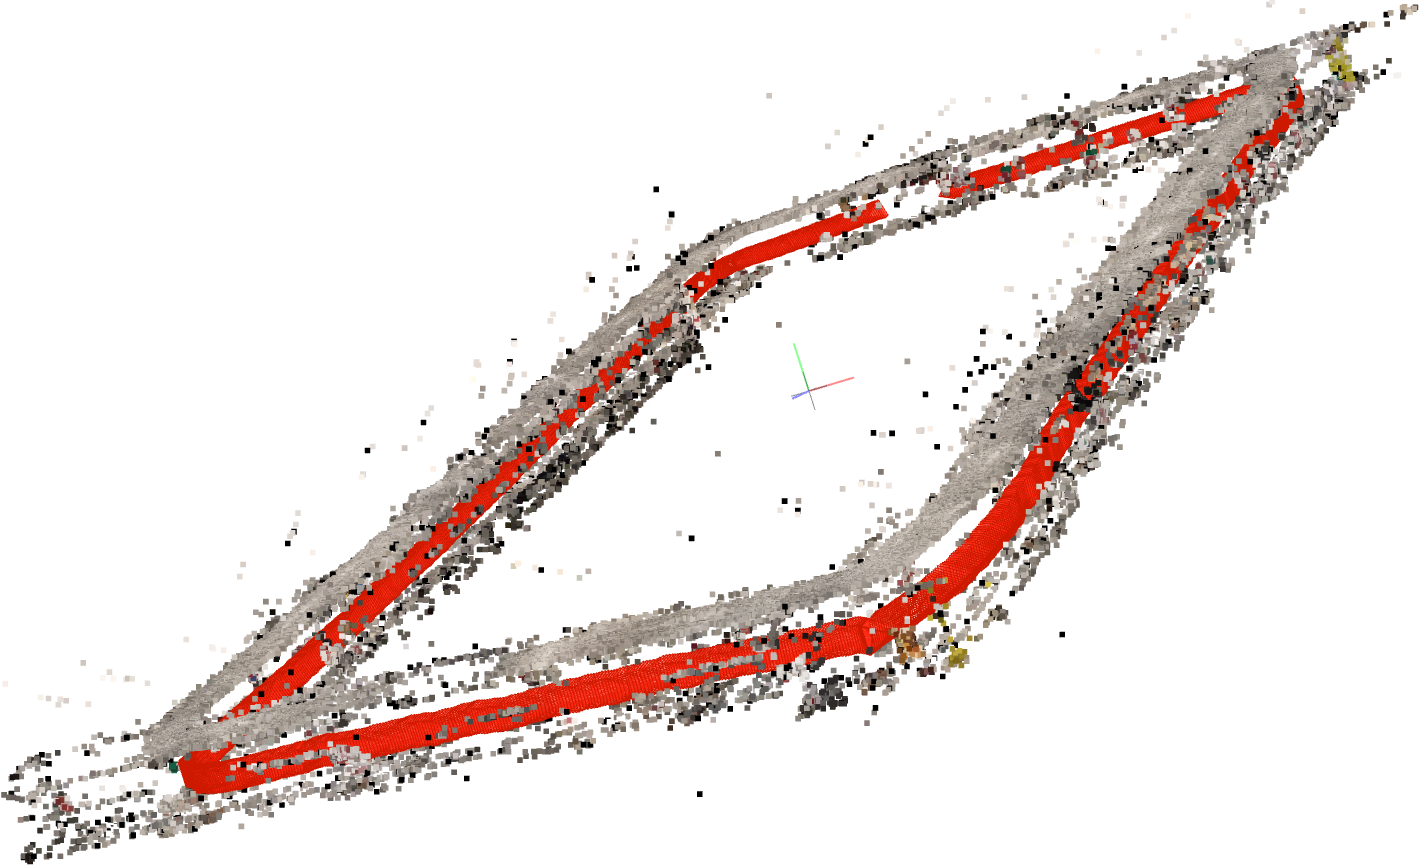
\includegraphics[width=0.45\textwidth]{./imgs/extracted_features_colmap.png}
    \end{center}
    \caption{Features extracted as a points clouds by COLMAP in the second floor of the Povo 1 building in the University of Trento. The red line represents the camera path in the video footage.}
    \label{fig:features-colmap}
\end{figure}

The set of poses is represented as a graph $\mathcal{G}=(\mathcal{V}, \mathcal{E})$ and for each node $i$ there is an association with a subset of environment features $\mathcal{F}_i : \mathcal{F}_i\subset P$. Edges in $\mathcal{E}$ connect poses from images that use common features.

The sparse reconstruction algorithm first extracts features from each given image and builds the set $P$, called also as \emph{bag of words}. Once this is done, thanks to a convolution on each image, it creates spacial associations between nodes in the graph comparing images with the bag of words. The convolution enables to map only subsections of the whole image: this allows to estimate the movement based on the position of the matrix used for the convolution within the image grid. Once associations are done, the features and the poses are composed in order to create the reconstructed model.

Moreover, the algorithm for the dense reconstruction is very similar to the one used for the sparse one. The main difference is about how the associations are created: in this case the algorithm uses point-wise associations and not convolutions. Even if it requires more computational resources, this approach allows to be more accurate and to create more definite point clouds.

Both algorithms can work on a sequence of unrelated photos of the same environment or a sorted sequence of frames: note that the reconstruction process is way more efficient in the second case.

\subsection{Coordinate reference system alignment}
The dataset generated by COLMAP has a \emph{coordinate reference system (CRS)} chosen arbitrarily during the reconstruction. Origin and axes of the COLMAP model may not coincide (actually this is always the case) with the real-world CRS. In order to align them, three steps are required:
\begin{enumerate}
    \item scale: it is necessary to scale the relative positions of the points with respect to the real-world CRS. This can be achieved measuring the distance between two known points in both COLMAP and real life;
    \item translation: align the origins;
    \item rotation: align the axes.
\end{enumerate}
The last two steps can be grouped together by using the euclidean or rigid transformation.
It involves a rotation $R$, a translation $t$ and at least three points for both the CRSs that represent the same locations. \Cref{eq:rigid-tranform} describes the rigid transformation:
\begin{equation}
    \begin{aligned}
        A & =\{(x_1^A, y_1^A), (x_2^A, y_2^A), (x_3^A, y_3^A)\} \\
        B & =\{(x_1^B, y_1^B), (x_2^B, y_2^B), (x_3^B, y_3^B)\} \\
        B & = R \times A+t
    \end{aligned}
    \label{eq:rigid-tranform}
\end{equation}

Matrix $R$ and vector $t$ are obtained using \textit{Singular Value Decomposition (SVD)}, it takes a matrix $E$ and return 3 other matrices, such that:
\begin{equation}
    \begin{aligned}
        [U, S, V] & = \textrm{SVD}(E) \\
        E         & = USV^T
    \end{aligned}
    \label{eq:singular-value-decomposition}
\end{equation}

To obtain the matrix $R$, the first step consists in aligning on the same origin the two datasets centroids. This is done by subtracting to each coordinate of each point the centroid of the respective dataset. After this, it is possible to ignore the translation component $t$ and compute the rotation $R$:
\begin{equation}
    \begin{aligned}
        H         & = (A-\textrm{centroid}_A)(B-\textrm{centroid}_B)^T \\
        [U, S, V] & = \textrm{SVD}(H)                                          \\
        R         & = VU^T
    \end{aligned}
    \label{eq:rotation-matrix}
\end{equation}

Finally, it is possible to use \cref{eq:rigid-tranform} to obtain the translation vector $t$:
\begin{equation}
    \begin{aligned}
        B =                   & R\times A + T                                     \\
        \textrm{centroid}_B = & R\times \textrm{centroid}_A + T                   \\
        t =                   & \textrm{ centroid}_B - R\times \textrm{centroid}_A
    \end{aligned}
    \label{eq:translation-vector}
\end{equation}
